\begin{slikaDesno}[0.83]{fig/rhp_zero.pdf}
    \textbf{\color{red}*}\PID У колу са слике познато је $C = 100\unit{nF}$, 
    $R_1 = 1\unit{k\Omega}$ и
    $G_{\rm m} = 1\unit{mS}$.
    Једини улаз посматраног система је напон 
    $v_{\rm U} = v_{\rm U}(t)$ а једини излаз је 
    $v_{\rm I} = v_{\rm I}(t)$.
    \begin{itemize}
    \item[(а)] 
    У општим бројeвима, 
    одредити функцију преноса, $H(s)$, датог 
    система
    и одредити полове и нуле те функције 
    преноса. 

    \item[(б)] 
    Израчунати у ком опсегу отпорности 
    $R_{\rm K}$ функција преноса $H(s)$
    има нулу у десној комплексној полуравни, 
    а у ком у
    левој комплексној полуравни.
\end{itemize}
\end{slikaDesno}
%
\begin{itemize}
    \item[(в)] За вредност отпорнисти 
    $R_{\rm K} = R_0$ за коју функција преноса 
    $H(s)$ 
    \myul{нема нула}, одредити одзив на побуду 
    $v_{\rm U}^{\text{(г)}} = 1\unit{V}\,{\rm u}(t)$
    применом Лапласове транформације.
    
    \item[(г)] На истом дијаграму, нацртати 
    одзив одређен у претходној тачки као и
    одзив система $H(s)$ за $R_{\rm K} = 0$ 
    на исту побуду. 
\end{itemize} 

\textsc{\underline{Решење}}: Функција преноса може се одредити применом методе 
потенцијала чворова, писањем једине једначине за излазни чвор 
\begin{equation}
    V_{\rm I} \left( \dfrac{1}{R_1} + \dfrac{1}{Z_{\rm K}} \right) = - G_{\rm m} V_{\rm U} + \dfrac{1}{Z_{\rm K}} V_{\rm U}, \label{\ID.eq1}
\end{equation}
где је $Z_{\rm K} = R_{\rm K} + \dfrac{1}{sC}$ уопштена комплкенсна импеданса гране са кондензатором. Преносна функција је 
у овом случају $H(s) = \dfrac{V_{\rm I}}{V_{\rm U}}$, па се сређивањем израза \ref{\ID.eq1} има облик 
\begin{equation}
    H(s) = \dfrac{sC(1 - G_{\rm m}R_{\rm K} ) - G_{\rm m} }{ sC\left(1 + \dfrac{R_{\rm K}}{R_1}\right) + \dfrac{1}{R_1} }. \label{\ID.eq2}
\end{equation}
Нуле функције преноса налазе се одређивањем коренова полинома у бројицу, а полови се налазе  одређивањем коренова полинома у имениоцу, чиме се 
налазе једина нула и једини пол функције преноса, у општем случају, дати изразима
\begin{equation}
    z = \dfrac{G_{\rm m}}{C(1 - G_{\rm m} R_{\rm K})}, \qquad \qquad p = - \dfrac{1}{C(R_1 + R_{\rm K})},
\end{equation}
редом.

(б) Знак нуле функције преноса $z = \dfrac{G_{\rm m}}{C(1 - G_{\rm m} R_{\rm K})}$, одређен је изразом
\begin{equation}
    \sgn z = \sgn {\dfrac{G_{\rm m}}{C(1 - G_{\rm m} R_{\rm K})}} = \sgn{(1 - G_{\rm m} R_{\rm K})}.
\end{equation}
Односно, уколико је $R_{\rm K} < \dfrac{1}{G_{\rm m}} = 1\unit{k\Omega}$, нула је у десној комплексној полуравни ($\Re{\sgn z} > 0$), док је 
за $R_{\rm K} > \dfrac{1}{G_{\rm m}} = 1\unit{k\Omega}$, та нула у левој комплексној полуравни ($\Re {\sgn z} < 0$). У нарочитом случају, 
када је $R_{\rm K} = \dfrac{1}{G_{\rm m}} = 1\unit{k\Omega}$, уколико погледамо у полазни резултат за функцију преноса \ref{\ID.eq2}, закључујемо да нуле функције преноса 
тада нема. Тада још кажемо и да је нула „померена у бесконачност“.

(в) Како је наглашено, када је $R_{\rm K} = R_0 = \dfrac{1}{G_{\rm m}} = 1\unit{k\Omega}$, функција преноса нема нула и тада је 
\small
\begin{equation}
    H(s) = - \dfrac{G_{\rm m} }{ sC\left(1 + \dfrac{1}{G_{\rm m} R_1}\right) + \dfrac{1}{R_1} } 
    = \dfrac{K}{1 + s\uptau}, \quad K = -G_{\rm m}{\rm R_1} = -1, \quad \uptau = C\left( R_1 + \dfrac{1}{G_{\rm m}} \right) = 200\unit{\upmu s},
\end{equation}
\normalsize
којом приликом је облик поједностављен увођењем константи $K$ и $\uptau$, чији су смисао статичко појачање и временска константа.  
Дата побуда у Лапласовом домену налази се применом табличне трансформације 
$\LT{\uu(t)} = \dfrac{1}{s}$, чиме се име $V_{\rm I} = \dfrac{V_0}{s}$, па се онда одзив налази на основу 
\begin{eqnarray}
    V_{\rm I}(s) = H(s) \cdot V_{\rm U}(s) = - \dfrac{V_{0}}{s} \cdot \dfrac{K}{1 + s\uptau}.
\end{eqnarray}
Добијени резултат у комплексном домену преводи се у комплкесни домен растављањем на парцијалне разломке, у облику 
\begin{eqnarray} 
    V_{\rm I}(s) = \dfrac{A}{s} + \dfrac{B}{1 + s\uptau} = 
    \begin{cases}
        A = \dfrac{V_{0}}{\xcancel{s}} \cdot  \dfrac{K}{1 + s\uptau}  \bigg|_{s = 0} = 
        K V_0 & \\[5mm]
        B =  
        \dfrac{V_{0}}{s} \cdot  \dfrac{K}{\xcancel{1 + s\uptau}}  \bigg|_{s = -1/\uptau} = -K \uptau V_0
        &.
    \end{cases}
\end{eqnarray}
Инверзном Лапласовом трансформацијом се онда налази резултат: 
\begin{equation}
    v_{\rm I}(t) = \ILT{V_{\rm I}} = K \ILT{ \dfrac{1}{s} + \dfrac{\uptau}{1 - s\uptau} } V_0 = 
    {K}(1 - \ee^{-t/\uptau} ) V_0 \, \uu(t)
\end{equation}

(г) На сличан начин као у претходној тачки, заменом $R_{\rm K} = 0$ у израз \ref{\ID.eq2} налази се 
\begin{equation}
    H(s) = \dfrac{s - \dfrac{G_{\rm m}}{C}  }{s + \dfrac{1}{C R_1}} = \dfrac{s - z}{s - p}, \quad \text{где су}, \quad
    z = +\dfrac{G_{\rm m}}{C}, \quad p = - \dfrac{1}{R_1 C}, 
\end{equation}
па се на сличан начин као у претходној тачки добија одзив у Лаплсовом домену
\begin{eqnarray} \small
    V_{\rm I}(s) = \dfrac{A}{s} + \dfrac{B}{s + p} = 
    \begin{cases}
        A = \dfrac{V_{0}}{\xcancel{s}} \cdot  \dfrac{s - z}{s - p}  \bigg|_{s = 0} = 
        \dfrac{z}{p} V_0 = - G_{\rm m} R_1 V_0 = K V_0& \\[5mm]
        B =  
        \dfrac{V_{0}}{s} \cdot  \dfrac{s - z}{\xcancel{s - p}}  \bigg|_{s = p} = \dfrac{p - z}{p} V_0 = (1 + G_{\rm m} R_1 ) V_0 = (1+K)V_0
        &.
    \end{cases}
\end{eqnarray}
У временском домену је онда $v_{\rm I}(t) = 
\left( K + (1-K) \ee^{-pt}  \right) V_0 \uu(t)$.
Заменом нумеричких резултата и цртањем одговарајућег графика добија се резултат који је приказан на слици 
\ref{\ID.f}.

\begin{figure}[ht!]
    \centering
    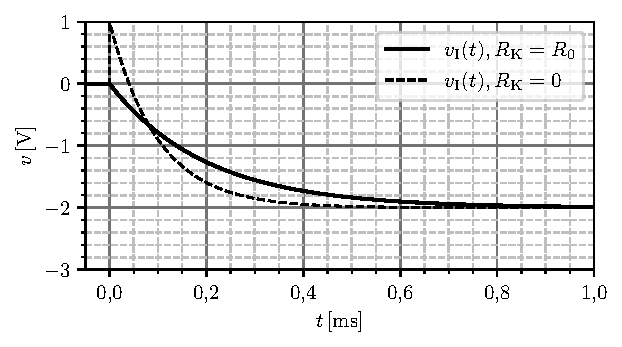
\includegraphics[scale=1]{fig/zero_rhs_plot.pdf}
    \caption{} \label{\ID.f}
\end{figure}

Прокоментаришимо добијене резултате. Нула у десној комплексној полуравни довела је до прекида одскочног одзива у тренутку побуде. Посебно, тај прекид је 
у \textit{супротну} страну од оног на коме ће одзив у бесконачности завршити. У овом конкретном случају, разлог за то јесте кондензатор повезан између улазног и излазног прикључка. 
Иако је статичко појачање система негативно, $K<0$, због самог постојања тог кондензатора, и његове немогућности да тренутно мења свој напон, 
у првим тренуцима ће излазни напон \textit{пратити} улазни напон, што доводи до оваквног одзива. Нижа временска константа тог процеса је последица 
мање отпорности коју „види“ кондензатор.

Односно, систем са нулом у десној комплексној полуравни ће у 
првим тренуцима реаговати на квалитативно другачији начин него касније. Ово може довести до проблема када се овакав систем користи у повратној спрези. 
Више речи о том ефекту тема су Линеарне електронике и теорије система аутоматског управљања. Иако је дугорочно понашање оба система практично исто 
(у бесконачности имају исту вредност), овај облик одзива значи да ће бити значајно теже контролисати систем са нулом у десној комплексној полуравни. 
Уметање отпорника $R_{\rm K} = R_0$ на ред са кондензатором $C$ представља \textit{компензацију}, и уклањање ове нуле из система.